\section{Evaluation}
\label{s:evaluation}

In this section, we conduct a thorough analysis of the effectiveness of Mazu's modules toward mitigating flow setup latencies. Ultimately, our goal is to understand whether Mazu can help SDN be more effective in providing fine time-scale control over network state.

\subsection{Inbound Latency}

We prototyped the proxy described in \S\ref{s:inbound} on a commodity host (Intel quad core CPU at 2.66Ghz and 8GB RAM). 
We evaluated it using the same setup as described in \S\ref{s:measure_inbound}. 
We found that the proxy almost completely eliminates the inbound delay: 
the delay is under 0.199ms (0.02ms) for a flow arrival rate of 200/s (2000/s); the 99th percentile delay is as small as 0.476ms (3.5ms), which is mainly due to the proxy's software overhead.  
 Since the proxy is physically decoupled from the switch, there is no impact of the switch's \flowmod\ or \packetout\ operations on the proxy's \packetin\ operations. 
In contrast, without the proxy, the mean and 99th percentile delays are 8ms and 192ms respectively, with a flow arrival rate of 200/s. 
These improvements are significant, especially for latency sensitive applications such as VoIP calls in cellular networks. 

% on average across various rates of incoming traffic. 

% We set the flow table of the switch to be empty so the openflow agent on the switch generates 
% the \packetin messages to the controller. We injected flows at the speed of 500/s, 1000/s and 2000/s and 
% time tamp when the packet is leaving the NIC of the host and when the \packetin messages are received by the openflow controller. 
% For each flow injection rate, we keep the experiments for 30 seconds. The average inbound delays for new flow arrival rate 500/s, 
% 1000/s and 2000/s are 0.0163, 0.0164 and 0.0189 ms respectively. 
% The 99.99\% percentile inbound delays for new flow arrival rate 500/s, 1000/s and 2000/s are 0.092, 1.938 and 3.489 ms, respectively.

 
\subsection{Outbound Latency} 
In what follows, we use a variety of large-scale simulations on various topologies with different workloads to study the impact of delays imposed by outbound latencies and the improvements offered by Mazu. We leverage the switch latency models derived from our measurements in \S\ref{s:outbound_meas}.

% We use our extensive measurement results from Broadcom and intel switch to derive a latency model as described in 
% section 6.1. From the measurement data sets we find the values of constant \textit{a}, \textit{b} and \textit{c} using curve fitting. We use these 
% values of  \textit{a}, \textit{b} and \textit{c} in our latency model to calculate the flow insertion completion time in our simulations.

\subsubsection{Macro Benchmarks}%Flow Engineering} 
\label{s:fe_eval}

To evaluate the effectiveness of Mazu's flow engineering technique, we simulate a failover scenario in a tunneled WAN network, where a random link experiences a failure. 

{\bf Topology: } We use a simple full mesh (overlay) network of 25 nodes.  The tunnels between these nodes share the same physical network. Each tunnel has between 5 and 10 intermediate switches. Per link capacity lies in $[100,1000]$.

{\bf Traffic matrix:} We assign a popularity index (random number) to each node. The number of flows between a pair of nodes is proportional to the product of their popularities. Each flow imposes a unit demand. At the start of our simulation, the traffic matrix is routed in a way such that the maximum load on any link is minimized.
% . The product of popularity index between any two nodes indicates the volume of traffic between them. Initially we map the generate traffic matrix to the network

{\bf Table occupancy:} We assume that the new rules being installed upon failure (some of these could be updates to existing rules) all have the same priority $P$. Further, we assume that the tunnel end-points already have some rules in them, a subset of which are displaced by the new rules. We randomly pick the number of such displaced rules within some interval (explained in more detail below). For simplicity, we assume that there are no dependencies across rules; we consider dependencies in subsequent sections.

\begin{table}
\centering
\small
\begin{tabular}{|c|c|c|c|}
\hline
{\bf Workload} & \tabincell{c}{ {\bf Popularity} \\{\bf Index}}  &\tabincell{c}{ {\bf Popularity Index } \\{\bf for high priority}\\ {\bf traffic}} & \tabincell{c}{ {\bf No of low} \\{\bf  priority rules} \\{\bf in the flowtable}}\\ \hline
s1 & 1-10 & 1-5 & 0-50 \\ \hline 
s2 & 1-10 & 1-5 & 100-200 \\ \hline
s3 & 1-10 & 1-5 &300-500 \\ \hline
s4 & 1-20 & 1-7 &0-50 \\ \hline
s5 & 1-20 & 1-7 &100-200 \\ \hline
s6 & 1-20 & 1-7 &300-500 \\ \hline
%\hline
\end{tabular}
\caption{Workloads used in simulation}{\label{qosTable}}
\end{table}


{\bf Workloads:} We consider six workloads (``s1'', ``s2'', ``s3'', ``s4'', ``s5'',  and ``s6'') shown in Table~\ref{qosTable}.  In low traffic workloads, s1, s2 and s3, the number of rules that can be displaced at any switch is in $[0,50]$, $[100,200]$, $[300,500]$ respectively; and the number of flows between any pair of nodes is on average 50 with a maximum of 100. In high traffic workloads, s4, s5 and s6, the number of rules that can be displaced at any switch is in $[0,50]$, $[100,200]$, $[300,500]$ respectively; and the number of flows between any pair of nodes is on average 200 with a maximum of 400.

% priority rules at each switch is between 20-50 and the ratio of traffic volume to link capacity is medium. In high workload, the number of low priority rules are in between 50-100 with a high traffic volume to link capacity ratio.

%  between 0 and $D$. \aditya{why not more?}

% assume that tunnel end points have rules already existing in them. The number of such rules and their priorities is picked at random. Thus, when a route is installed on such a switch, some of these rules may be displaced. \aditya{priorities correct? which rules are displaced??}

To simulate failures we randomly select a tunnel in the mesh and fail it. We assume that there is enough spare capacity in the network to route the affected traffic.

We study three  mechanisms: (a) Base case, which re-routes the affected flows while minimizing the maximum link load, ignoring setup latencies.%  This is akin to the heuristic outlined in \S\ref{s:floweng} except that we don't consider rule installation latency at all. 
(b) Flow engineering (FE) to select paths for affected flows such that flow installation latency is minimized (\S\ref{s:floweng}). (c) Flow Engineering and Rule Offload (FE + RO), which  implements rule offloading (\S\ref{s:offload})  in addition to FE. It offloads a set of rules from the tunnel end-nodes to at most $k=3$ next hop switches per tunnel. 

In all cases, we assume that one-shot consistent updates are employed to install routes. Thus, our metric of interest is the {\em worst case latency incurred at any switch to install all new/modified routes at the switch.}

On a link failure, around 70 flows get rerouted for low traffic workloads and 220 for high traffic workloads. All the rerouted flows are treated as new flows.  
%  For our simulations we have considered a nominal value for k (=3).     

% For both (b) and (c) above we assume that optimal rule update is employed (\S\ref{s:optimal}). Our results are averaged across the various links we failed in the simulations.

% Once this failure scenario is simulated we use the following three techniques independently to allocate affected flows to existing paths.

% We assume that the base case failover recovery algorithm will try to use the link with maximum available free space to 
% accommodate the flows on the failed links in a greedy fashion. It does not consider the number of rules to be installed or the table occupancy on the 
% switches in the path selection. For our evaluation we use a full mesh (overlay) network of 25 nodes in which all nodes are interconnected via 
% tunnels. The tunnels share the same physical network and have 5-10 intermediate physical switches. and also assign random table occupancy to the nodes to account for rule 
% displacement costs when some new rules are inserted. To simulate failures we randomly select any tunnel and fail it. We assume that there is enough 
% space to adjust the affected traffic otherwise the routes has to recompute for all the flows. Once this failure scenario is simulated we use the 
% following three techniques independently to allocate affected flows to existing paths.

% \begin{itemize}

% \item The base case greedy technique which allocates the affected flows in decreasing order of link capacities.
% \item The Mazu FE technique which allocates the affected flows considering the latencies imposed by the rule insertions.
% \item The Mazu FE + Flow Offload technique which applies Flow offloading to the flows allocated by the Mazu FE algorithm to offload a set of rules from the nodes to at most k next hop physical switches in the tunnel to reduce the 
% maximum number of rule insertions at any switch. For our simulations we have considered a nominal value for k (=3).    
% \end{itemize}

% We use our latency model to find the total flow completion time for all the above scenarios. For a flow F of priority P to be installed at any node N 
% there are some random number (x) of rules already in N that have priority P', where P > P' so that the installation of F will cause the displacement 
% of x rules. Each displacement of rule will add to the latency of insertion of F and our latency model will calculate it. For our simulations, the 
% factor x varies from 0 to 100.

% We consider three workloads (low, medium and high). In case of low workload, we have at random 0-20 low 
% priority rules at each switch and the traffic volume to link capacity 
% ratio is also low. In medium workloads the number of low 
% priority rules at each switch is between 20-50 and the ratio of traffic volume to link capacity is medium. In high workload, the number of low priority rules are in between 50-100 with a high traffic volume to link capacity ratio. 

We simulate both with Broadcom and Intel, assuming all switches in the network are from the same vendor.


% We use Broadcom switch latency model to calculate the latencies incurred in failover recovery scenario with the above workloads. 

Figure~\ref{failoverResults} shows the latencies with Broadcom switches for the three techniques. For the lowest volume workload, the base case incurs a latency of 720ms, whereas FE improves this to 259ms and FE+RO to 133ms. These improvements are crucial, especially for latency sensitive interactive applications.

For the rest of the workloads, base case latency varies between 2 and 14s. Using FE offers 22-35\% improvement, but using FE together with RO leads to nearly a {\em factor of 3} improvement in all cases. Note that the gains can be improved further by: (1) leveraging more core switches for offload, (2) providing a modest amount of reserved capacity for highly critical traffic, so that during failures the number of flows whose routes have to be recomputed is small and the rerouted non-critical flows can tolerate modest amounts of downtime or congestion. In other words, Mazu provides operators additional flexibility in designing schemes to better meet failover requirements in their networks.

% workloads of low traffic volume (s1, s2, s3), the latency-agnostic base case incurs latencies of nearly 721 ms for the s1 workload (with low table occupancy), and nearly 5.5 s for s3 workload (with high table occupancy). In contrast, for similar workloads, Mazu's FE improves the worst case latency at any switch by nearly 22-35\%. Adding RO provides further substantial improvements; the worst case latency is about 1.9 s for s3, i.e., a net improvement of {\em nearly a factor of 3}. We see similar improves for the high traffic workloads (s4, s5, s6).
% \aditya{takeaway???}

%  the latency-agnostic approach incurs of nearly 2.4 secs for s4 workload (with low table occupancy), and nearly 14.4 secs for s6 workload (with high table occupancy). Whereas, with Mazu's FE+RO technique the worst case latency decreases by 60.4\%(5.7 sec),

% \aditya{comment on takeaway}

We also run our simulation with the Intel switch model. Recall that all rules we insert have the same priority. Since the Intel switch does not 
impose rule displacement in such situations, the latency is purely driven by the maximum number of rules inserted at any switch. In our simulations, 
this is almost always at source end-point on a failed tunnel. Since both base case and FE are equally impacted by this, we don't see any improvement 
from using FE. However, RO still applies, as rules can be offloaded to core switches---we see an improvement of {\em over 2X} (324ms to 129ms).

% we don't observe improvements from using FE in our specific setting because FE won't reduce the max number of rules to be inserted at the edge switch. But with rule offloading we still observe an improvement of 50\% 

 
% \aditya{talk about results for Intel?}
% Our simulation with broadcom switch model shows that low priority rule displacement(table occupency) has a significant effect on overall flow set up time. FE reduces the flow installation time by selecting the paths with low latencies. The effectiveness of FE is further improved by RO which brings about further reduction in completion time by factor of nearly 2.5-3 times.    


% significantly high especially in the high workload. Mazu's FE techniques bring an improvement of nearly 30\% in all the scenarios by considering the number of rules to be inserted and the table occupancy on switches. The FE + Rule Offload technique proves to be even more effective in bringing an improvement of almost 66-72\% which shows its effectiveness in spreading the rule across the network to control latencies.

\begin{figure}[!tb]
\centering
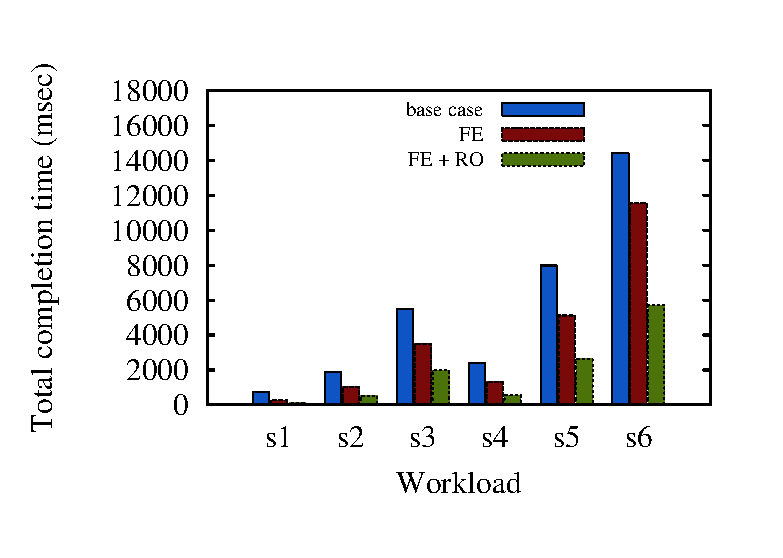
\epsfig{file=./figs/Failover.eps,width=0.35\textwidth}
\vspace{-1em}
\compactcaption{ Worst case flow setup time of affected flows in failover scenario with base case, FE and FE+RO techniques in a full mesh (25 nodes) topology with Broadcom switches }\label{failoverResults}
\end{figure}


\subsubsection{Micro Benchmarks}%Rule Offload in Depth} 

{\bf ClassBench:} While the above scenarios did leverage rule offload, the rules inserted had a flat priority structure and did not have dependencies. In what follows, we study how well rule offload works when these simplifying criteria may not apply.  We leverage ClassBench~\cite{classbench} to generate a variety of rule sets representative of real world access control. Since dependent rule sets in most cases hinder rule offloading to the next hops switches we believe that the ACL rule sets generated from ClassBench--which have a significant amount of dependencies--will present a near worst case scenario for our rule offload scheme.

% \begin{figure}[!tb]
% \centering
% %%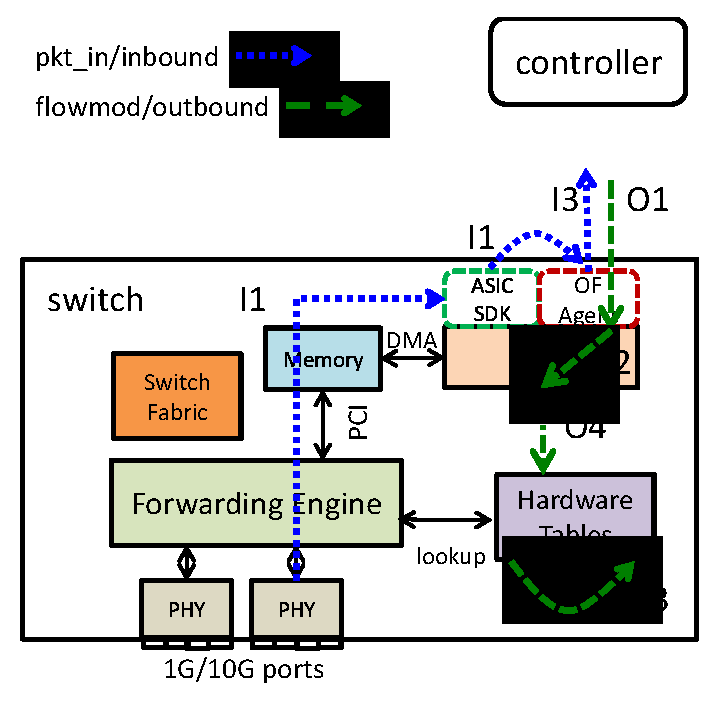
\epsfig{file=./figs/openflow_switch_illustrate.eps,width=0.35\textwidth} %%changed
% 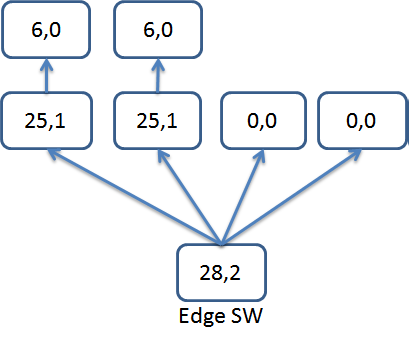
\includegraphics[width=2.5in]{figs/ruleoffload_cb.png}
% \caption{rule offloading from an edge switch with 90 rules to its
% next hops. The numbers a,b (e.g. 28,2) denotes the number of rooted
% rules and default rules
% respectively. }\label{experiment_setup} \end{figure} 


We consider the following simple setup: we use a three-level FatTree topology~\cite{fattree-sigcomm08} with degree 8, containing 128 servers connected by 32 edge switches, 32 aggregate switches and 16 core switches.  We use ClassBench to generate 90 rules for each edge switch. Each rule is assigned a different priority and a tunnel tag to indicate its tunnel or path. 

Without rule offloading, assuming one-shot updates, the installation time will be the maximum at any edge switch when inserting 90 rules. Under rule offload, we assume that a core switch cannot accommodate more than 60 rules in total from {\em all} of its immediate upstream neighbors.

We experimented with a variety of rule sets generated by ClassBench. On average, we found that the speedup from using rule offload relative to not using it is 2.1 for Broadcom switches and 1.4 for Intel switches. This speedup is made possible by rule offload ``spreading'' out rules to downstream switches, enabling parallel execution of updates. 

% To show how rule offload works, we present the distribution of the
% offloaded and default rules across the network in Figure
% ~\ref{classbenchResults}. The switch IDs from 0-31 denote the edge
% switches, each having 90 rules to be inserted, 32-63 denote
% aggregate switches and 64-89 denote core switchs. Figure shows the
% overall rule distribution of accross the network as a result of rule
% offload.   

% We apply the rule offloading algorithm on each of the rule sets to
% generate the partitions to offload the rules. Once the partitions
% are generated for the switches each containing rules of differing
% priorities to be installed on that switch, we calculate the total
% insertion latencies incurred in the best case scenario (increasing
% order for Intel and decreasing order for broadcom) to insert those
% rules . We repeat this experiment for  different rule set generated
% using Class Bench and then calculate the average completion
% time. Since, all the offloaded rules and the remaining rules at the
% edge switches can be inserted in parallel, this technique proves to
% be very effective in reducing the overall rule insertion completion
% time. In our simulations, we observe that the speed up in completion
% time for topology with Broadcom and  Intel switches to be 2.1 and
% 1.4 respectively. 

% \begin{figure}[!tb]
% \centering
% 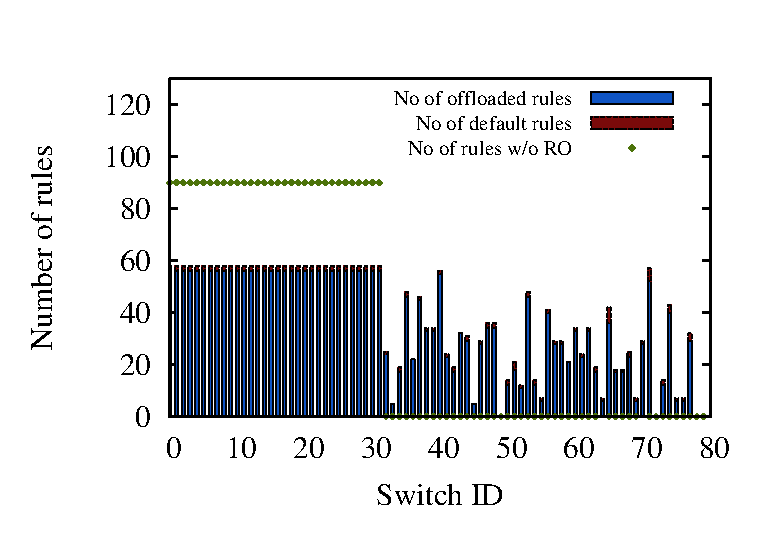
\epsfig{file=./figs/ClassBench_RuleDist1.eps,width=0.4\textwidth}
% \caption{ Rule offloading using ClassBench rules on Fat Tree topology (k=8). Distribution of rules across the network }\label{classbenchResults}
% \end{figure}

{\bf MicroTE:} We now consider an important scenario discussion in \S\ref{sec-motivation}, namely fine-grained intra-DC traffic engineering using MicroTE~\cite{microte}. MicroTE leverages the partial and short term predictability of the traffic matrix in a datacenter to perform traffic engineering at small time-scales.  As noted in \S\ref{s:floweng}, FE does not apply to MicroTE since routes span a single tunnel and route changes all happen at a single switch. Thus, MicroTE can only benefit from rule offload, the extent of which we study next.




% We examine the performance of our flow offloading module under varying levels of workloads. We use MicroTE, a traffic 
% engineering application, to evaluate the performance for an independent rule set, and class bench to generate real world rule sets with dependent 
% rules.


% {\bf Rule offload without dependencies}

% We use MircoTE to examine the effectiveness of rule offload on a 
% rule set without dependencies.
We use the same data center topology as discussed earlier in this section. We assume that the traffic rate between a pair of servers is derived from a Zipfian distribution.  Figure ~\ref{microteResults} shows the rule installation completion time. We see that RO provides a 2X improvement (400ms to 200ms) assuming the Broadcom switch. Given the time-scales of predictability considered, this can help MicroTE leverage traffic predictability longer, thereby achieving more optimal routing. The improvement in case of Intel is 1.6X (80ms to 48ms).

%  MircoTE with flow offloading has 40\% improvement with intel's switch model and 50\% with broadcom's witch model in overall competition time.

\begin{figure}[!tb]
\centering
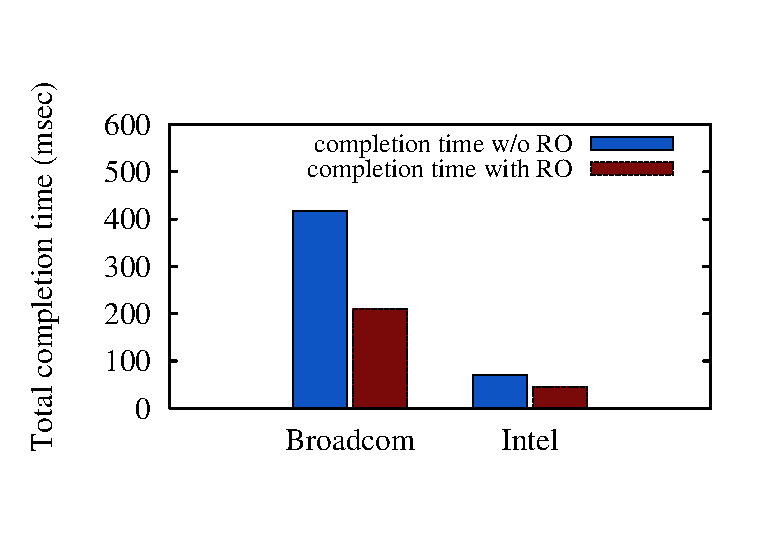
\epsfig{file=./figs/MicroTE_Compl.eps,width=0.35\textwidth}
\vspace{-1em}
\compactcaption{ Flow setup time of MicroTE with and without RO in a Fat Tree (k=8) topology}\label{microteResults}
\end{figure}

\subsubsection{Two-level Responsive Traffic Engineering} 

Our experiments above evaluated individual components of Mazu in isolation. Next, we consider a network management application where FE and RO (with priority handling) both come into play.

Our application is a two-level responsive traffic engineering scheme
whose goal is to simultaneously route two categories of traffic --
high and low priority --
according to different objectives over the same underlying network.
This could apply to an ISP that deploys (two classes of) service
differentiation. The question we address here is how quickly can the network
establish routes when requests arrive closely in time for both
categories of traffic. The faster this is, the
closer the network's ability to meet the SLAs for the corresponding
classes. This experiment underscores the ability of Mazu to
help applications that desire fine-grained state control in order
to meet complex objectives.


To emulate this, in a somewhat simplistic fashion, we use different objective functions to route each category. For routing low priority traffic, the 
objective is to minimize the overall link utilization of the network due to this traffic. We install coarse grained (wildcard) rules in the switch 
to route this traffic. The objective for higher priority traffic is to minimize the overall link cost, where cost of a link could be  latency. To route the high priority traffic we install fine grained high priority rules. These fine grained rules could overlap with the coarse 
grained rules and when they do, they have higher rule priority. At first we
route the low priority traffic, and then on the remaining network capacity we route the high priority traffic. For simplicity we assume that both categories of traffic can be 
accommodated without causing any congestion. The rest of the setup is same as
in \secref{s:fe_eval}. The high and low priority traffic 
between any pair of nodes is proportional to their respective ``popularity'' indices (we assign popularity to the nodes at random 
in the range as shown in \tabref{qosTable}). For high volume workloads (s4, s5 and s6) the volume of high priority and low priority traffic between any two 
overlay nodes is about 17 and 200 flows, respectively, and for low volume
workloads (s1, s2 and s3) the volume is about 12 and 50 flows, respectively.


% We use 25 nodes full mesh overlay network, where each node pair is connected via a virtual tunnel, to simulate this situation.


% We used the same topology for simulating our TE+QoS application and for simulating our failover. As before, also in this simulation, both high and 
% low priority traffic between a pair of overlay nodes is proportional to the popularity of the node (we assign popularity to nodes at random). In our 
% simulations, we first investigated the performance gain of just applying flow engineering on high priority traffic, and then we investigated the 
% performance gain of applying flow engineering on the high priority traffic along with using flow offload for both classes of traffic. We examine the 
% performance improvement of rule offloading and rule engineering on our TE application under different types of workload.  In particular, we consider 
% three different types of workloads, shown in 


\figsref{qos_Results}{qos_intelResults} show the total completion time using
Broadcom and Intel switches, respectively, with and without our techniques. The base case has a significantly high flow set up time when the number of low priority rules in the table are high: as high as 80s for Broadcom. This implies that ignoring flow setup latency can cost traffic engineering dearly in terms of being responsive.  For low volume workloads (s1, s2, s3) the factor of improvement from just FE is about 2.5X for Broadcom and 1.8X for Intel, and is about 5X for Broadcom and 4X for Intel with FE+RO. We observe similar speedups for high volume workloads (s4, s5, s6). 

We conclude that all the mechanisms in Mazu are crucial to ensuring that the
route setup is sufficiently fast for management applications that desire
fine-grained control to achieve complex objectives.




\begin{figure}
% \subfloat[Flow rate = 100/s, concurrent with \flowmod\ and \packetout\ \label{fig:intel_inbound_test1}]
%   {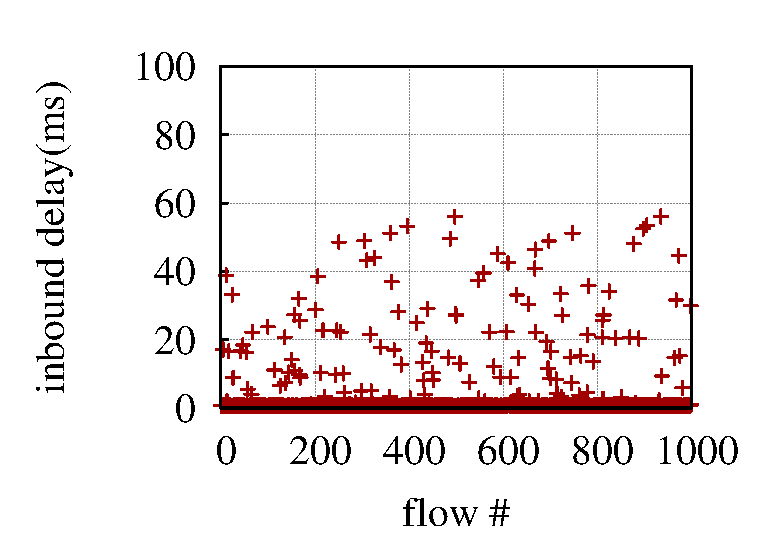
\includegraphics[width=.33\linewidth]{./figs/jan27_intel_inbound_with_pktout_flowmod_rate100.eps}}\hfill
%\subfloat[Flow rate = 200/s\label{fig:hp_inbound_test2}]
%  {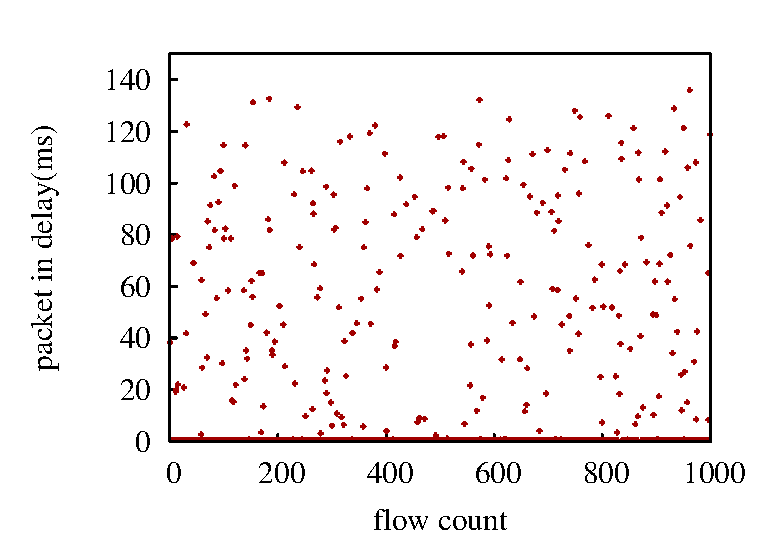
\includegraphics[width=.28\linewidth]{./figs/hp_inbound_delay_200.eps}}\hfill
\subfloat[Latency on Broadcom switch \label{qos_Results} ]
  {\includegraphics[width=.5\linewidth]{./figs/qos.eps}}
\subfloat[Latency on Intel switch \label{qos_intelResults} ]
  {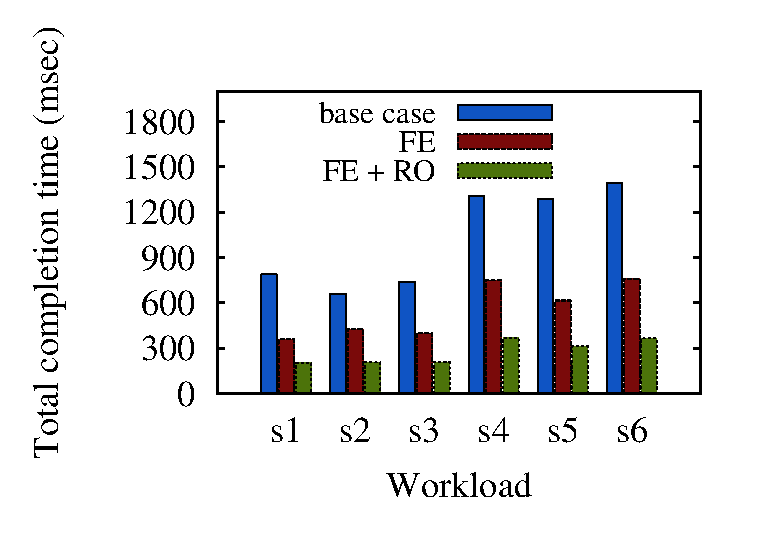
\includegraphics[width=.5\linewidth]{./figs/qos_intel.eps}}
  \vspace{-5pt}
\caption{Worst case flow set up time of two level traffic engineering scheme with base case, FE and FE+RO techniques in a full mesh topology with 25 nodes}
\label{qosResults}
\end{figure}

\iffalse

\begin{figure}[!tb]
\centering
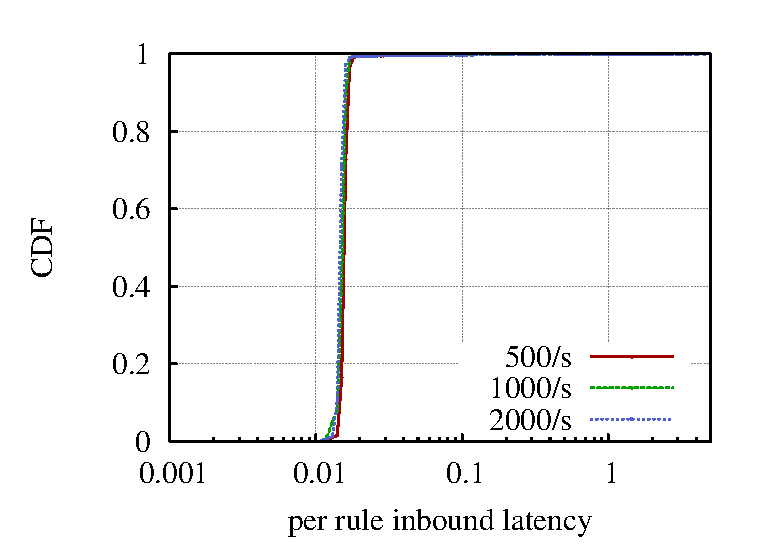
\epsfig{file=./figs/MB_perf_HP.eps,width=0.3\textwidth}
\caption{Evaluating MB's performance using HP procurve 8212zl openflow switch.}\label{MB_perf_hp}
\end{figure}


\begin{figure}[!tb]
\centering
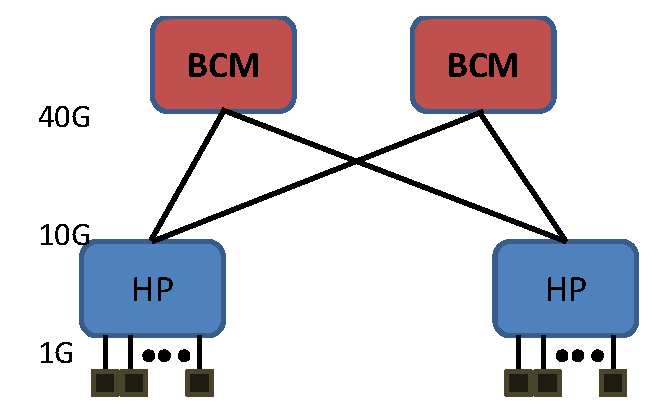
\epsfig{file=./figs/eva_testbed.eps,width=0.35\textwidth}
\caption{Testbed.}\label{testbed}
\end{figure}

\fi



%\begin{figure}[!tb]
%\centering
%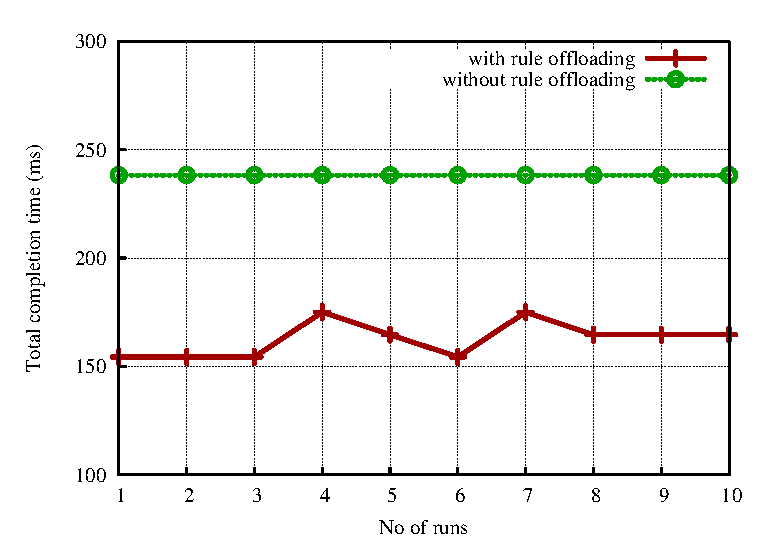
\epsfig{file=./figs/Classbench_RuleOffload2.eps,width=0.42\textwidth}
%\caption{Evaluating Rule offloading using ClassBench rules on Fat Tree topology (k=8). Effect on total completion time of rule insertions }\label{testbed}
%\end{figure}


%\begin{figure}[!tb]
%\centering
%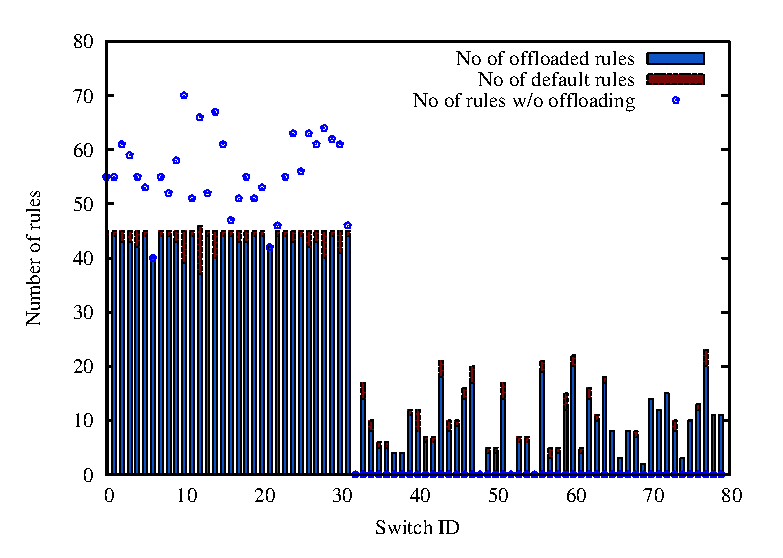
\epsfig{file=./figs/MicroTE_Dist.eps,width=0.42\textwidth}
%\caption{ Rule offloading using rules generated from MicroTE on Fat Tree topology (k=8). Distribution of rules across the network }\label{testbed}
%\end{figure}


\iffalse
metrics for evaluating ingress and egress latency reduction techniques:

\begin{itemize}

\item extent of reduction in latency
\begin{itemize}

\item testbed 

\begin{enumerate} 
\item single switch: ingress delay

- change flow rate

- change rule complexity

\item simple topology with K (=2 or 3) paths each of length L (= 2 or 3) hops between a pair of nodes: ingress and egress delay

- change flow rate

- change rule complexity

- show how effective different ideas as (multi-table + multipath; multi-table + flow engineering)

\end{enumerate}

\item simulations

\begin{enumerate} 

\item rocketfuel topologies: assume switches are homogeneous. assume we have switch latency as a function of rule size (from our measurements - we can use these directly to model latencies in our simulation); assume simple rules with uniform priority

- draw flow rates from a distribution: flow rate between two nodes in the topology proportional to product of populations of nodes (indicating traffic skew)

- use switch latency functions to impose the appropriate latency on every switch.

- study improvement in egress and ingress delays

\item Assume rules with different priorities: draw priorities from a Zipf distribution (with a small number of priority values)

- draw flow rates from same distribution as above

- study improvement in egress and ingress delays

\end{enumerate}

\end{itemize}

\item Impact in specific application scenarios

\begin{itemize}

\item intra-DC traffic engineering

- fat-tree topology

- DC traffic traces used in MicroTE

- switch latency models same as before

- Improvement in maximum link utilization from using our egress delay management technique vs ignoring it completely
 
\item failover  (Li)
- similar setting as intra-DC TE
- Reduce congestion time and increase link utilization during failover via
controller fast reroute 
- need an algorithm, modify SWAN?

\item mobility (Li)
- use softCell synthetic fat tree topology
- compare path setup with and without our techniques

\end{itemize}

\end{itemize}


* a given topology and given workload

topology

traffic mix

rule granularity/complexity

\fi

